%%%%%%%%%%%%%%%%%%%%%%%%%%%%%%%%%%%%%%%%%%%%%%%%%%%%%%%%%%%%%%%%%%%%%%%%%%%%%%%%
%% 

\chapter{Anforderungen, Systemarchitektur und Datenmodell} \label{sec:requirements_architecture}
\section{Anforderungen}
\label{sec:requirements}
Basierend auf den in Kapitel~\ref{sec:related_work} vorgestellten Systemen sowie konkreten Anforderungen des Krankenhauses wurden die Systemanforderungen definiert. Während \textcite{nabeshimaASPbasedNurseScheduling2026} Dienstpläne im Vier-Wochen-Rhythmus mit einer Vielzahl an Schichttypen erstellen und \textcite{alvianoNurseReschedulingAnswer2019} Jahrespläne mit drei Schichtarten optimieren, beschränkt sich die vorliegende Arbeit bewusst auf eine einheitliche Tagesschicht sowie eine monatliche Planungsperiode. Der Fokus liegt dabei nicht auf der Optimierung des ASP-Encodings für große Instanzen, sondern auf der vollständigen Integration in eine  Fullstack-Webanwendung mit interaktiver Benutzeroberfläche. Analog zu \textcite{nabeshimaASPbasedNurseScheduling2026} wird das System als webbasierter Dienst bereitgestellt und unterstützt neben der initialen Planung ein Rescheduling bei kurzfristigen Ausfällen. Ein wesentliches Merkmal gegenüber allen verglichenen Systemen ist die vorausschauende Berechnung von Alternativplänen, die eine Absicherung gegen zukünftige Ausfälle ermöglicht. In Tabelle~\ref{tab:technologien} wird die genaue Technologie des jeweiligen Subsystems erläutert.
\begin{table}[h]
	\centering
	\caption{Verwendete Technologien}
	\label{tab:technologien}
	\begin{tabularx}{\linewidth}{l>{\raggedright\arraybackslash}Xl}
		\toprule
		\textbf{Subsystem} & \textbf{Technologie} & \textbf{Version} \\
		\midrule
		\texttt{Frontend}   & Angular                & 21.2.6 \\
		\texttt{Backend}    & FastAPI                & 0.135.3 \\
		\texttt{Datenbank}  & PostgreSQL / Supabase  & 15.1 \\
		\texttt{ASP-Solver} & Clingo                 & 5.8.0 \\
		\bottomrule
	\end{tabularx}
\end{table}

Das System soll die Erstellung eines Monatsplans von der Pflegeleitung für die Mitarbeiter einer Krankenhausabteilung ermöglichen. Für jeden Mitarbeiter soll die Anzahl der Arbeitstage pro Monat erfasst werden können. Im Rahmen dieser Arbeit wird ausschließlich eine Tagesschicht betrachtet, unterschiedliche Schichtarten werden daher nicht berücksichtigt.

Zusätzlich müssen verschiedene harte Constraints eingehalten werden. Ein Mitarbeiter darf an einem Tag nur einer Station zugeteilt werden. Außerdem darf eine Zuteilung nur erfolgen, wenn der Mitarbeiter über die erforderlichen Kompetenzen für die jeweilige Station verfügt. Bestimmte Zuteilungen von Mitarbeitern zu Tagen und Stationen sollen als fixiert markiert werden können, sodass diese bei einer Neuberechnung des Plans unverändert bleiben. Ebenso soll definiert werden können, dass ein Mitarbeiter an bestimmten Tagen nicht eingeteilt werden darf, oder an bestimmten Tagen eingeteilt werden muss.

Neben den verpflichtenden Einschränkungen sollen auch weiche Constraints berücksichtigt werden. Als weicher Constraint wurde eine möglichst faire Verteilung der Mitarbeiter auf die einzelnen Stationen definiert. Wenn eine gültige Lösung existiert, bei der jede Station an jedem Tag mit mindestens einem Mitarbeiter besetzt ist, soll das System eine möglichst gleichmäßige Zuteilung der Mitarbeiter auf die Stationen anstreben.

Ein weiterer wichtiger Aspekt ist die Berechnungszeit des Systems. Vergleichbare Systeme, wie jene von \textcite{alvianoNurseReschedulingAnswer2019} und \textcite{cardellini2023solvingrehabilitationschedulingproblems}, erstellen Dienstpläne innerhalb weniger Minuten. Das entwickelte System soll daher ebenfalls in der Lage sein, einen Monatsplan in einem vergleichbaren Zeitrahmen zu berechnen. Gleiches gilt für ein krankheitsbedingtes \textit{Rescheduling}.



\section{Systemarchitektur}
Die Applikation besteht aus einer dreischichtigen Architektur, die in Angular-Frontend, FastAPI-Backend sowie einer Supabase-Datenbank mit PostgreSQL aufgeteilt wird. Die Daten zu Stationen, Mitarbeitenden und Kompetenzen sind synthetisch generierte Testdaten. Sie orientieren sich hinsichtlich ihrer Struktur und der verwendeten Attribute an typischen Daten eines Krankenhauses, wurden jedoch vollständig künstlich erstellt. Insbesondere wurden die Namen von Mitarbeitenden generiert und es wurden keine realen personenbezogenen oder krankenhausspezifischen Daten verwendet. Die Abbildung \ref{fig:Applikations-Architektur} stellt die Schichten grafisch dar.
\begin{figure}[h]
	\centering
	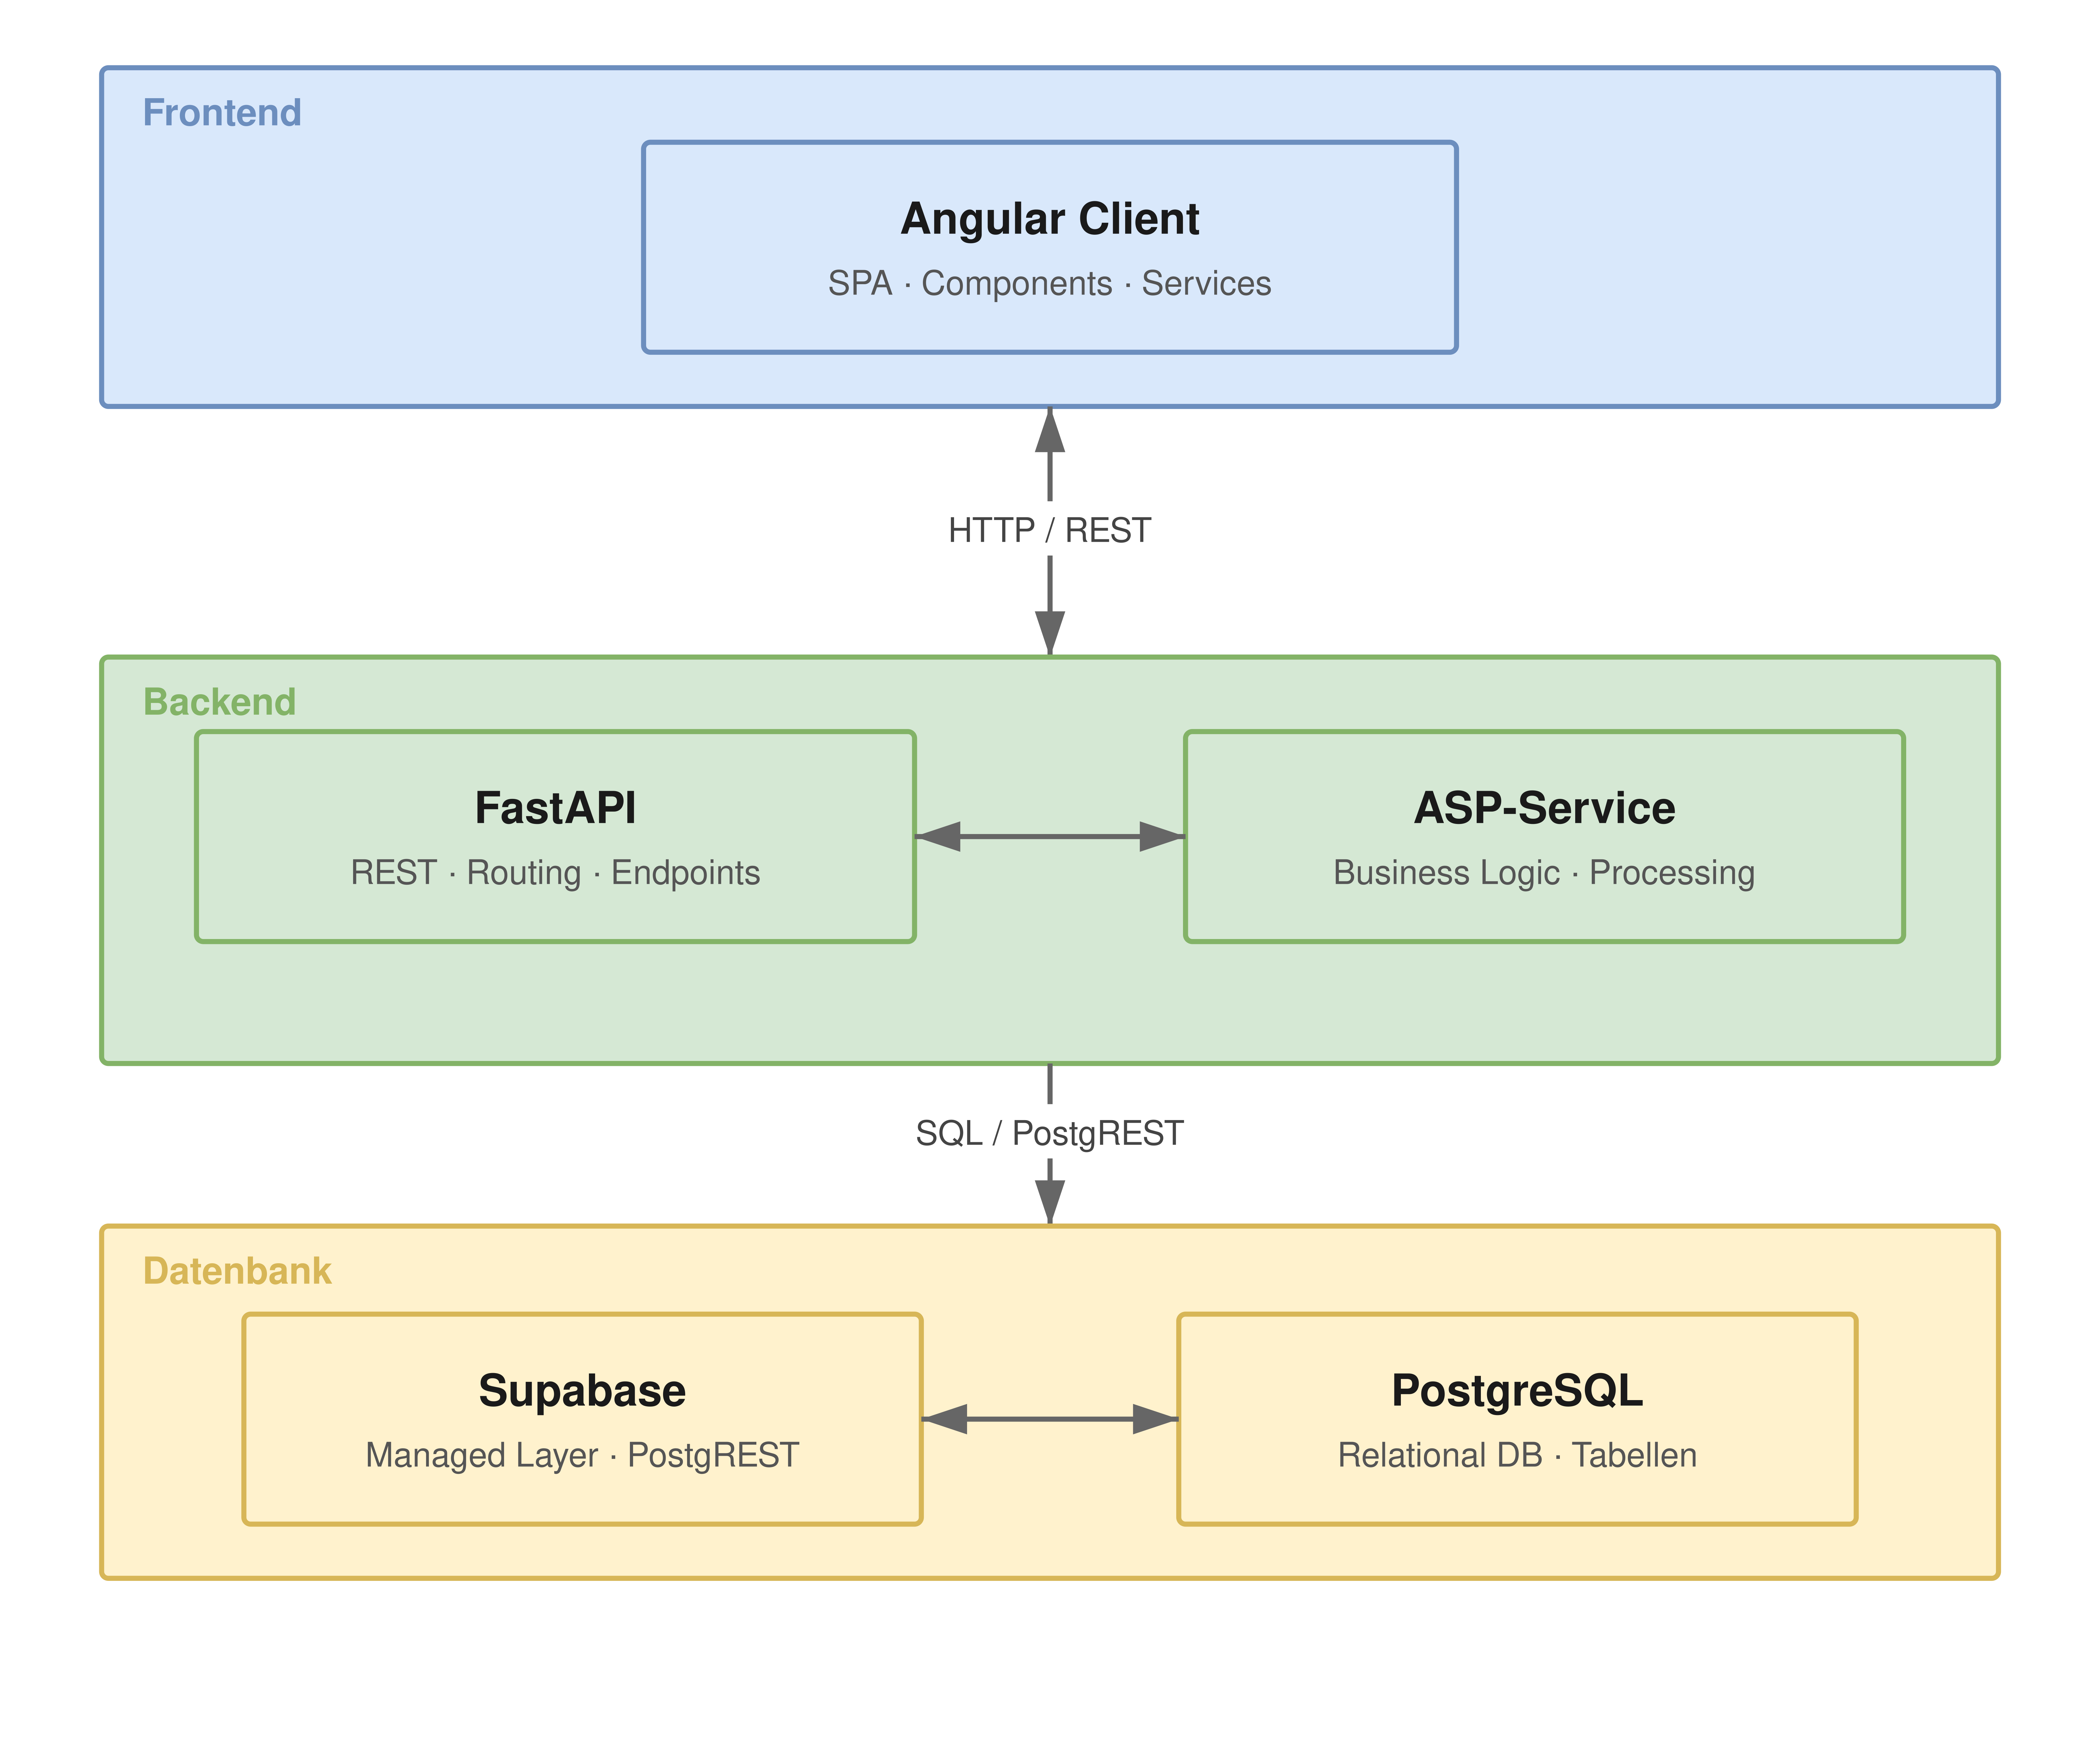
\includegraphics[width=\linewidth]{figures/architecture}
	\caption{
		Applikations-Architektur
	}\label{fig:Applikations-Architektur}
\end{figure}

Das Frontend wurde als Single-Page Application mit dem Angular Framework umgesetzt. Es stellt die Benutzeroberfläche bereit, über die Mitarbeiter, Stationen und Kompetenzen verwaltet, sowie Constraints festgelegt und Monatspläne angezeigt werden können. Die Kommunikation mit dem Backend erfolgt ausschließlich über HTTP-REST-Schnittstellen.
Das Backend ist in Python mit FastAPI realisiert und übernimmt die gesamte Geschäftslogik der Anwendung. Es stellt REST-Endpunkte bereit und verarbeitet eingehende Anfragen. Ein zentraler Bestandteil des Backends ist der ASP-Service. Dieser Service ist für die Berechnung der Monatspläne unter Berücksichtigung der definierten Hard und Soft Constraints verantwortlich.
Als Datenbankschicht wird Supabase eingesetzt, eine Open-Source-Plattform, die auf PostgreSQL aufbaut. Supabase stellt neben der relationalen Datenbank auch eine PostgREST-Schnittstelle bereit, über die das Backend direkt auf die Datenbankressourcen zugreifen kann.

\section{Datenmodell}

Das Datenmodell bildet die Grundlage für die Speicherung und Verwaltung der im System benötigten Informationen. Es wurde als relationales Datenbankschema umgesetzt und besteht aus mehreren Entitäten, die als Datenbanktabellen realisiert sind. Neben den zentralen Tabellen zur Abbildung von Mitarbeitenden, Kompetenzen, Stationen und Dienstplänen enthält das Modell verschiedene Assoziationstabellen zur Darstellung von Beziehungen zwischen diesen Entitäten. Die Struktur sowie die Beziehungen der einzelnen Tabellen sind in der Abbildung \ref{fig:Datenmodell} dargestellt. Im Folgenden werden die einzelnen Tabellen und ihre Zusammenhänge näher erläutert.

\subsection{Entitäten}

Die Tabelle \texttt{users} repräsentiert die Mitarbeitenden des Systems. Neben dem Primärschlüssel \texttt{id} wird der Name eines Mitarbeitenden im Attribut \texttt{name} gespeichert. Die Tabelle dient als zentraler Bezugspunkt für Qualifikations- und Zuweisungsbeziehungen.

Die Tabelle \texttt{skills} bildet die im System verfügbaren Kompetenzen ab. Jede Kompetenz wird durch eine eindeutige \texttt{id} sowie einen \texttt{name} beschrieben.

Die Tabelle \texttt{stations} modelliert die Arbeitsstationen, denen Mitarbeitende zugewiesen werden können. Das Attribut \texttt{maxAssignments} definiert die maximale Anzahl gleichzeitiger Zuweisungen pro Station und stellt somit eine wesentliche Kapazitätsbeschränkung dar.

Die Tabelle \texttt{schedules} dient der Verwaltung von Dienstplänen. Über die Attribute \texttt{year} und \texttt{month} können Dienstpläne zeitlich eingeordnet werden. Das Attribut \texttt{is\_loaded} speichert, welcher Dienstplan aktuell im Kalender geladen ist.

\subsection{Assoziationstabellen}

Die Tabelle \texttt{user\_skills} stellt die Zuordnung zwischen den Tabellen \texttt{users} und \texttt{skills} her. Dadurch kann gespeichert werden, über welche Qualifikationen ein Benutzer verfügt, wobei einem Benutzer mehrere Fähigkeiten zugewiesen sein können und eine Fähigkeit wiederum mehreren Benutzern zugeordnet werden kann. Die Tabelle besteht ausschließlich aus den beiden Fremdschlüsseln \texttt{user\_id} und \texttt{skill\_id}.

Die Tabelle \texttt{station\_skills} definiert die für eine Station erforderlichen Qualifikationen und stellt die Verbindung zwischen den Tabellen \texttt{stations} und \texttt{skills} her. Eine Station kann dabei über mehrere notwendige Qualifikationen verfügen. Diese Informationen ermöglichen anschließend den Abgleich zwischen den Fähigkeiten der Benutzer und den Anforderungen der jeweiligen Stationen.

Die Tabelle \texttt{station\_assignments} stellt die zentrale Verknüpfung des Datenmodells dar. Sie ordnet für ein bestimmtes Datum (\texttt{date}) eine Station (\texttt{station\_id}) einem Benutzer (\texttt{user\_id}) sowie einem Dienstplan (\texttt{schedule\_id}) zu. Das Attribut \texttt{user\_id} ist optional, sodass auch Zuweisungen ohne konkreten Benutzer gespeichert werden können. Dies ermöglicht die Abbildung von Platzhalterzuweisungen für den Fall, dass einem Dienstplan nicht für jede Station unmittelbar ein Mitarbeiter zugeordnet werden kann. Der \textit{Unique Constraint} auf den Spalten \texttt{schedule\_id}, \texttt{date} und \texttt{user\_id} stellt dabei sicher, dass ein Benutzer eines Dienstplans pro Tag nur einer einzigen Station zugewiesen werden kann.
\begin{figure}[h]
	\centering
	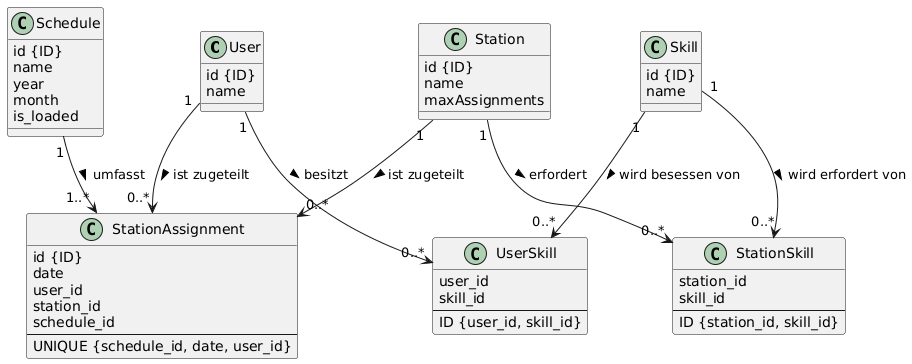
\includegraphics[width=\linewidth]{figures/datenmodell_plantuml}
	\caption{
		Datenmodell
	}\label{fig:Datenmodell}
\end{figure}

%% 
%%%%%%%%%%%%%%%%%%%%%%%%%%%%%%%%%%%%%%%%%%%%%%%%%%%%%%%%%%%%%%%%%%%%%%%%%%%%%%%%
